\documentclass[]{article}
\usepackage{fontspec}
%\setmainfont{Arial}[ItalicFont={Arial Italic}]
%\setmainfont{Gill Sans MT}[ItalicFont={Gill Sans MT Italic}]
\usepackage[utf8]{inputenc}
\usepackage[margin=1.5cm, bindingoffset=1cm]{geometry}
\linespread{1.5}
\usepackage{float}
\usepackage{csquotes}
\usepackage{subfig}
\usepackage{graphicx}
\usepackage{wrapfig}
\usepackage{xcolor}
\usepackage{indentfirst}
\setlength{\parindent}{0cm}
\usepackage[italian]{babel}
\usepackage{amsmath,amssymb}
\usepackage{hyperref}
\usepackage{amsmath}
\usepackage{enumerate}
% Imposto colore hyperlinks
\hypersetup{
    colorlinks=true,
    linkcolor=blue,
    urlcolor=blue,
    }
\usepackage{color}
\usepackage{listings}
\usepackage{wrapfig}
\usepackage{url}

\lstset{showstringspaces=false}

\title{CCFDetector}
\author{Marco Santoriello}
\date{Gennaio 2024}

\begin{document}
\begin{titlepage}
    \begin{center}
        \LARGE{\uppercase{Università degli Studi di Salerno}}\\
        \vspace{5mm}
        %Dipartimento
    	\uppercase{\normalsize Dipartimento di Informatica}\\
    \end{center}
    \begin{figure}[H]
        \centering
        
\includegraphics[width=0.35\textwidth]{img/logo_unisa.png}
    \end{figure}

    \begin{center}
        %Corso di Laurea
    	\normalsize{ Corso di Laurea in informatica }\\
    	\vspace{15mm}
    	%Titolo
        {\LARGE{\bf CCFDetector: Using ML against Credit Card Frauds }}\\
        {\large{ Progetto realizzato per l'esame di Fondamenti di Intelligenza Artificiale}}\\
    	\vspace{10mm}
    \end{center}
    \begin{minipage}[t]{0.4\textwidth}\raggedright
        %Candidato
    	{\large{Scritto da: \\ \bf Marco Santoriello\\ Mat. 0512114100}}
    \end{minipage}

    \vspace{90mm}
    %Anno Accademico
    \centering{\large \uppercase{ Anno Accademico 2023/2024 }}

\end{titlepage}

\setcounter{tocdepth}{3} %IMPOSTO LIVELLO PROFONDITA' INDICE

\tableofcontents
\newpage


\section{Introduzione}
    Negli ultimi anni, sempre più piede hanno preso i pagamenti elettronici, al punto che, anche in Italia, per legge, ogni commerciante deve essere munito di un dispositivo che permetta al cliente di pagare utilizzando la propria carta di credito, rischiando, in caso di mancato adempimento a questa legge, ingenti sanzioni pecuniarie.\\
    Come è facile immaginare, questo cambiamento nel modo in cui il denaro viene messo in circolazione ha interessato notevolmente criminali e truffatori (i cosiddetti \textit{scammers}), i quali hanno trovato non pochi modi di impossessarsi illecitamente, in maniera fisica o meno, delle carte di credito altrui.
    Basti pensare che negli Stati Uniti, secondo la \textit{Federal Trade Commission}, la tipologia di furti di identità più diffusi è proprio correlata alle frodi relative alle carte di credito.\\
    Queste frodi possono avvenire in svariati modi: si parte dal furto vero e proprio della carta di credito, fino ad arrivare, tramite diversi metodi, all'appropriazione dei soli dati della carta che abilitano al pagamento, passando per la clonazione delle carte e per l'utilizzo di dispositivi \textit{contactless} in posti affollati in prossimità dei portafogli delle ignare vittime.\\
    Questo progetto nasce con lo scopo di addestrare un modello di Machine Learning che permetta una facile ed affidabile individuazione delle transazioni fraudolente.

    \subsection{Specifica PEAS}
        La specifica PEAS (Performance, Environment, Actuators, Sensors) è un sistema che permette di descrivere l'ambiente operativo di un agente intelligente. L'obiettivo principale del progetto è quello di massimizzare la capacità dell'agente di rilevare transazioni fraudolente. L'ambiente in cui l'agente dovrà operare è di seguito descritto:
        \begin{itemize}
            \item Performance:
            \item Environment:
            \item Actuators:
            \item Sensors:
        \end{itemize}

    \subsection{Caratteristiche dell'ambiente}
        % TO-DO

    \subsection{Analisi del Problema}
        %TO-DO

\section{Data Understanding}
    \subsection{Data Collection}
        Definito il Problem Statement, passo all'individuazione del dataset adatto per l'addestramento e la validazione del modello.\\
        Trattandosi di dati particolarmente sensibili, il numero di dataset presenti online non è molto alto. Il primo \href{https://www.kaggle.com/datasets/mlg-ulb/creditcardfraud}{dataset} ritenuto particolarmente interessante per gli scopi di questo progetto, risultava avere quasi tutte le features criptate (per ovvi motivi di privacy) e delle quali non veniva fornita alcuna spiegazione, trattandosi di transazioni reali, rivelandosi non ottimale in termini di explainability.
        La scelta è poi ricaduta su un \href{https://www.kaggle.com/datasets/ealtman2019/credit-card-transactions/data}{dataset} contenente dati simulati, rilasciato da IBM.

    \subsection{Data Description}
        Il dataset in questione comprende dati, ottenuti attraverso un processo di simulazione che non è stato reso noto, di oltre 24 milioni di transazioni, di cui 30.000 fraudolente (cioè lo 0.1\%). Essendo dati simulati, ci si aspetta siano fedeli rappresentazioni delle transazioni reali e delle loro caratteristiche.\\
        Le features di questo dataset comprendono tutti i dettagli relativi a un pagamento elettronico (ID utente, ID carta, data, ora, modalità di pagamento, ecc.) e tutti i dettagli del venditore (i cui nomi sono stati codificati). La variabile target è rappresentata dalla colonna \textit{Is Fraud?}.\\
        Per ragioni legate alla capacità dell'hardware, decido di caricare soltanto 300.000 righe del dataset, verificando subito la presenza di transazioni fraudolente tra quelle importate.
        Procedo, a questo punto, con la documentazione dei dati.\\
        La prima cosa che noto è che le colonne \textit{Merchant State}, \textit{Zip}, ed, in particolare \textit{Errors}, contengono dei valori nulli.
        \begin{figure}[H]
            \centering
            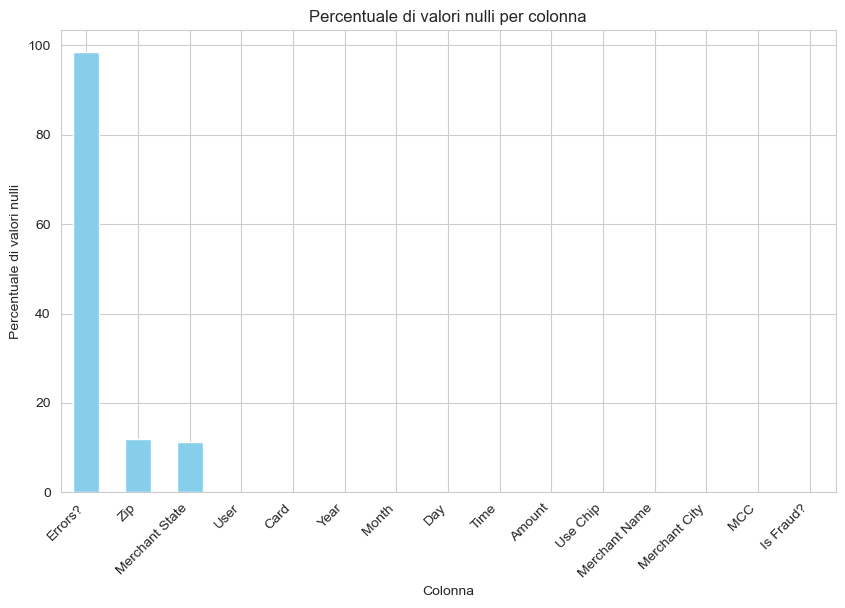
\includegraphics[width=.6\textwidth]{img/NullValuesPercentage.png}
            \caption[short]{Percentuale valori nulli per colonna}
        \end{figure}
        Inoltre, le caratteristiche \textit{Merchant State} e \textit{Zip} possono essere ricavate da \textit{Merchant City}, dunque potrebbe essere conveniente, contenendo valori nulli, rimuoverle. Ci sono poi caratteristiche, come Time, Amount e la variabile target che sarebbe conveniente avere come interi.


\end{document}